\documentclass[a0,plainsections,30pt]{sciposter}\usepackage[]{graphicx}\usepackage[]{color}
%% maxwidth is the original width if it is less than linewidth
%% otherwise use linewidth (to make sure the graphics do not exceed the margin)
\makeatletter
\def\maxwidth{ %
  \ifdim\Gin@nat@width>\linewidth
    \linewidth
  \else
    \Gin@nat@width
  \fi
}
\makeatother

\definecolor{fgcolor}{rgb}{0.345, 0.345, 0.345}
\newcommand{\hlnum}[1]{\textcolor[rgb]{0.686,0.059,0.569}{#1}}%
\newcommand{\hlstr}[1]{\textcolor[rgb]{0.192,0.494,0.8}{#1}}%
\newcommand{\hlcom}[1]{\textcolor[rgb]{0.678,0.584,0.686}{\textit{#1}}}%
\newcommand{\hlopt}[1]{\textcolor[rgb]{0,0,0}{#1}}%
\newcommand{\hlstd}[1]{\textcolor[rgb]{0.345,0.345,0.345}{#1}}%
\newcommand{\hlkwa}[1]{\textcolor[rgb]{0.161,0.373,0.58}{\textbf{#1}}}%
\newcommand{\hlkwb}[1]{\textcolor[rgb]{0.69,0.353,0.396}{#1}}%
\newcommand{\hlkwc}[1]{\textcolor[rgb]{0.333,0.667,0.333}{#1}}%
\newcommand{\hlkwd}[1]{\textcolor[rgb]{0.737,0.353,0.396}{\textbf{#1}}}%
\let\hlipl\hlkwb

\usepackage{framed}
\makeatletter
\newenvironment{kframe}{%
 \def\at@end@of@kframe{}%
 \ifinner\ifhmode%
  \def\at@end@of@kframe{\end{minipage}}%
  \begin{minipage}{\columnwidth}%
 \fi\fi%
 \def\FrameCommand##1{\hskip\@totalleftmargin \hskip-\fboxsep
 \colorbox{shadecolor}{##1}\hskip-\fboxsep
     % There is no \\@totalrightmargin, so:
     \hskip-\linewidth \hskip-\@totalleftmargin \hskip\columnwidth}%
 \MakeFramed {\advance\hsize-\width
   \@totalleftmargin\z@ \linewidth\hsize
   \@setminipage}}%
 {\par\unskip\endMakeFramed%
 \at@end@of@kframe}
\makeatother

\definecolor{shadecolor}{rgb}{.97, .97, .97}
\definecolor{messagecolor}{rgb}{0, 0, 0}
\definecolor{warningcolor}{rgb}{1, 0, 1}
\definecolor{errorcolor}{rgb}{1, 0, 0}
\newenvironment{knitrout}{}{} % an empty environment to be redefined in TeX

\usepackage{alltt}

\usepackage{graphicx}
% \usepackage{subcaption}
\usepackage{caption}

\usepackage{epstopdf, graphicx}
\usepackage{booktabs,dcolumn}
\usepackage{amsmath}
\usepackage{amsthm}
\usepackage{amssymb}
\usepackage{bbm}
\usepackage{hhline}
\usepackage{multicol}
\setlength{\columnseprule}{0pt}

\usepackage{boxedminipage}

\newcommand{\widgraph}[2]{\includegraphics[keepaspectratio,width=#1]{#2}}

\newcommand{\Rbb}{\mathbb{R}}
\newcommand{\Expect}{\mathbb{E}}
\newcommand{\Expecthat}{\hat{\mathbb{E}}}
\newcommand{\Var}{\text{Var}}
\newcommand{\Cov}{\text{Cov}}
\newcommand{\vbfamily}{\mathcal{Q}}
\newcommand{\etaopt}{\eta^{*}}
\newcommand{\etazopt}{\eta_z^{*}}
\newcommand{\etathetaopt}{\eta_\theta^{*}}
%\newcommand{\qopt}{q^{*}}
\newcommand{\targethat}{\hat{g}}
\newcommand{\QExpect}
{\Expect_{q\left(\theta, z \vert \eta_\theta, \etazopt(\eta_\theta)\right)}}
\newcommand{\atzero}{\Big\rvert_{\eta_\theta = \etathetaopt, \epsilon = 0}}
\newcommand{\etathetalin}{\eta_\theta^{LIN}}

\usepackage[framemethod=TikZ, xcolor=RGB]{mdframed}

\definecolor{mydarkblue}{rgb}{0,.06,.5}
\definecolor{mydarkred}{rgb}{.5,0,.1}
\definecolor{myroyalblue}{rgb}{0,.1,.8}

\usepackage{sectsty}
\sectionfont{\color{mydarkblue}\centering\LARGE\bf}

\mdfdefinestyle{MyFrame}{%
    linecolor=mydarkblue,
    outerlinewidth=2pt,
    roundcorner=20pt,
    innertopmargin=10pt,
    innerbottommargin=10pt,
    innerrightmargin=10pt,
    innerleftmargin=10pt,
    backgroundcolor=blue!10}


\title{\textcolor{mydarkblue}{Evaluating Sensitivity to the Stick Breaking Prior in Bayesian Nonparametrics
}}
% \usepackage{authblk}
% \author[1]{Author A}
% \author[1]{Author B}
% \author[1]{Author C}
% \author[1]{Author D}
% \author[2]{Author E}
% \affil[1]{Department of Computer Science, \LaTeX\ University}
% \affil[2]{Department of Mechanical Engineering, \LaTeX\ University}

\author{Ryan Giordano\textsuperscript{1*} \quad 
Runjing Liu\textsuperscript{1*} \quad 
Michael I. Jordan\textsuperscript{1} \quad 
Tamara Broderick\textsuperscript{2} \\
{\large\normalfont\textsuperscript{*} These authors contributed equally}\\
 {\large\normalfont\textsuperscript{1} Department of Statistics, UC Berkeley \quad \textsuperscript{2} Department of EECS, MIT}
 }

\leftlogo[1]{images/logo_left.png}
\rightlogo[1]{images/logo_right2.png}

% Set the color used for the section headings here
\definecolor{SectionCol}{rgb}{0,.06,.5}
\definecolor{lightblue}{rgb}{0.8,0.8,1}

% Set some fbox commands line width and the color we use in the f boxes
\setlength{\fboxrule}{.09cm}
\definecolor{boxcolor}{rgb}{1,1,1}
\definecolor{innerboxcolor}{rgb}{.9,.94,.98}

% Math macros
\newcommand{\eq}[1]{Eq.~(\ref{eq:#1})}

\newcommand{\kl}{\textrm{KL}}
\newcommand{\mbe}{\mathbb{E}}
\newcommand{\mbeq}{\mathbb{E}_{q}}
\newcommand{\var}{\textrm{Var}}
\newcommand{\cov}{\textrm{Cov}}
\newcommand{\iid}{\stackrel{iid}{\sim}}
\newcommand{\indep}{\stackrel{indep}{\sim}}
\newcommand{\gauss}{\mathcal{N}} % Gaussian distribution

\DeclareMathOperator*{\argmin}{arg\,min}

% \newcommand{\npp}{\tilde{\eta}} % natural parameter for the p distribution
% \newcommand{\npq}{\eta} % natural parameter for the q distribution
% \newcommand{\mpp}{\tilde{m}} % mean parameter for the p distribution
% \newcommand{\mpq}{m} % mean parameter for the q distribution
% \newcommand{\mpopt}{m^*} % mean parameter for the q^* distribution
% \newcommand{\npopt}{\eta^*} % mean parameter for the q^* distribution
% \newcommand{\truecov}{\Sigma} % True posterior covariance
% \newcommand{\lrcov}{\hat{\Sigma}} % LR cov estimate
% \newcommand{\vbcov}{V} % Variational posterior covariance
% \newcommand{\constant}{C} % A constant

% my added commands
\usepackage{etoolbox}
\BeforeBeginEnvironment{figure}{\vskip-2ex}
\AfterEndEnvironment{figure}{\vskip-1ex}

% Fiddle with the margin
\addtolength{\topmargin}{-0.5in}
% \addtolength{\topmargin}{-0.875in}
\addtolength{\textheight}{1in}
\IfFileExists{upquote.sty}{\usepackage{upquote}}{}
\begin{document}
\conference{NIPS 2017}


\setlength{\parskip}{0.25em}

\maketitle

\vspace{-1in}


\newcommand{\bnpalpha}{2}
\newcommand{\betamean}{0.38}
\newcommand{\betainfo}{0.10}
\newcommand{\gammascale}{0.10}
\newcommand{\gammashape}{10.00}
\newcommand{\bmean}{0}
\newcommand{\binfo}{0.10}
\newcommand{\nboot}{200}
\newcommand{\kapprox}{30}
\newcommand{\nobs}{1000}
\newcommand{\betadim}{7}
\newcommand{\ntime}{14}
\newcommand{\splinedegree}{3}





%%%%%%%%%%%%%%%%%%%%%%%%%%%%%%%%%
%%%%%%%%%%%%%%%%%%%%%%%%%%%%%%%%%
% FIRST COLUMN
%%%%%%%%%%%%%%%%%%%%%%%%%%%%%%%%%
%%%%%%%%%%%%%%%%%%%%%%%%%%%%%%%%%
%\columnbreak

\begin{minipage}[t]{0.45\textwidth}

\begin{mdframed}[style=MyFrame]
%%%%%%%%%%%%%%%%%%%%%%%%%%%%%%%%%
%%%%%%%%%%%%%%%%%%%
\section*{Overview}
\vspace{-0.3in}
%%%%%%%%%%%%%%%%%%%
%%%%%%%%%%%%%%%%%%%%%%%%%%%%%%%%%
\begin{itemize}
\item Researchers often want to estimate the number of clusters present in a dataset. 

\item A Bayesian nonparametric (BNP) model makes inferring the number of clusters amenable to Bayesian inference. 

\item We approximate the exact posterior with variational Bayes. 

\item \textbf{Question}: how sensitive is the
VB approximation, and the resulting inferences, to BNP model choices? 

\item \textbf{Problem}: re-running VB for multiple model choices is expensive. 

\item \textbf{We propose}: a linear approximation to efficiently
estimate BNP sensitivity from a single run of VB (to avoid
expensive refitting). 

\item We evaluate sensitivity to parametric and functional perturbations. 

\end{itemize}
\end{mdframed}
\vspace{-0.7in}

%%%%%%%%%%%%%%%%%%%%%%%%%%%%%%%%%
%%%%%%%%%%%%%%%%%%%
\section*{Model and inference }
\vspace{-0.3in}
%%%%%%%%%%%%%%%%%%%
%%%%%%%%%%%%%%%%%%%%%%%%%%%%%%%%%

The \textbf{Dirichlet process} is a popular Bayesian nonparametric
(BNP) model used for clustering.  

\begin{figure}[!h]
\centering
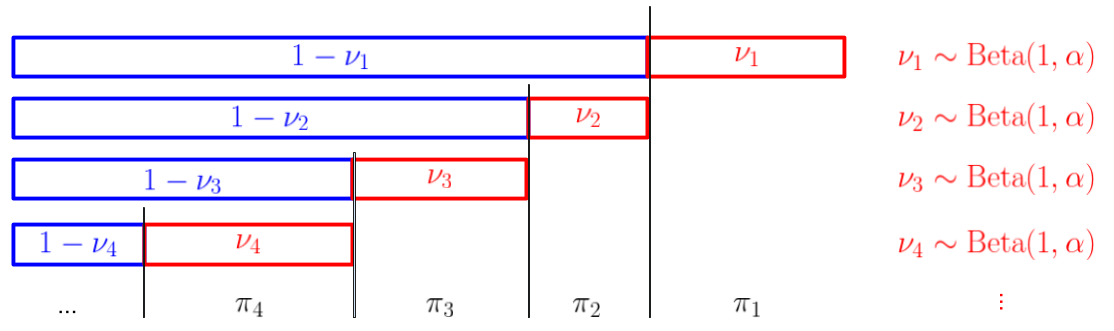
\includegraphics[width = 0.95\textwidth]{./images/DP_stick_breaking.png}
\caption{The Dirichlet stick-breaking process. We start with a stick of
length 1, and recursively break off proportions $\nu_1$, $\nu_2$, $\nu_3$, ...
The weights on the components are the lengths broken off at each step.}
\setlength{\textfloatsep}{-10pt}
\end{figure}

%%% iris figure
% \begin{figure}[!h]
% \centering
% 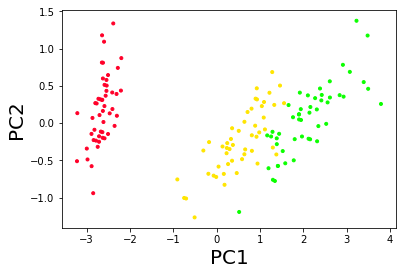
\includegraphics[width = 0.7\textwidth]{./images/iris_data.png}
% 
% \caption{The iris data projected onto the first two principal components. Color corresponds to the true iris species. }
% 
% \setlength{\textfloatsep}{-10pt}
% \end{figure}

We approximate the true posterior using \textbf{variational Bayes} (VB). Let $\eta^*$ denote the optimal variational parameters.
% 
% Note that: 
% 
% \begin{itemize}
% 
% \item The optimal variational parameters $\eta^*$ depend on the prior through optimizing the KL objective. 
% 
% \item All approximate posterior quantities (e.g.\ the expected number of clusters) are functions of $\eta^*$. 
% 
% \end{itemize}

\begin{mdframed}[style=MyFrame]
- How does varying the distribution $\nu_k \sim \text{Beta}(1, \alpha)$ affect $\eta^*$?

- While VB is fast, refitting for multiple choices of the DP prior would be
computationally prohibitive.

- {\bf Hence, we propose a linear approximation, derived from local sensitivity measures. }
\end{mdframed}

% Our objective is then 
% \vspace{-0.2in}
% \begin{align}
% \etathetaopt =
% \argmin_{\eta_\theta} KL\left(
%     q(\theta, z \vert \eta_\theta, \etazopt(\eta_\theta) \big\| p(\theta, z | y)
%     \right)
%     \label{eq:kl_objective}
% \end{align}

% \vspace{-0.7in}

% %%%%%%%%%%%%%%%%%%
% \subsection*{Posterior expectations of interest: }
% \vspace{-0.3in}
% %%%%%%%%%%%%%%%%%%
% We consider two possible posterior quantities:
% 
% \begin{enumerate}
% \item An {\bf in-sample quantity}, the expected number of clusters in the given iris dataset.
% % \vspace{-0.3in}
% % \begin{align}
% % \Expect_{q(z \vert \etazopt(\etathetaopt))} \left[ \#\{\text{distinct clusters}\} \right]
% % \label{eq:expected_num_clusters_thresh}
% % \end{align}
% 
% \item A {\bf posterior predictive quantity}, or the number of clusters we expect see in a \textit{new} dataset of $N$ iris flowers, given our posterior knowledge.
% % \begin{align}
% % \Expect_{q(\nu \vert \etathetaopt)} 
% % \left[\#\{\substack{\text{distinct clusters}\\\text{in new dataset}}\} \right] 
% %     \label{eq:expected_num_clusters_pred_thresh}
% % \end{align}
% 
% \end{enumerate}

%%%%%%%%%%%%%%%%%%%%%%%%%%%%%%%%%
%%%%%%%%%%%%%%%%%%
\vspace{-0.6in}
\section*{Hyperparameter sensitivity}
\vspace{-0.3in}
%%%%%%%%%%%%%%%%%%
%%%%%%%%%%%%%%%%%%%%%%%%%%%%%%%%%

\begin{itemize}

\item Let $\epsilon$ be a real-valued hyperparameter for the stick-breaking distribution
(e.g., this could be the $\alpha$ concentration parameter). 

\item The optimal VB parameters $\eta^*$ depend on $\epsilon$ through optimizing the KL objective. 

\item The expected number of clusters depend on $\eta^*$. Can use either an in-sample or a predictive quantity, 
\vspace{-0.1in}
\begin{align}
\Expect_{q_{\eta^*}} \left[ \#\{\text{distinct clusters}\} \right]
\quad \text{ or } \quad 
\Expect_{q_{\eta^*}} 
\left[\#\{\substack{\text{distinct clusters}\\\text{in new dataset}}\} \right].
\end{align}
\end{itemize}

%%%%%%%%%%%%%%%%%%%%%%%%%%%%%%%%%
%%%%%%%%%%%%%%%%%%%%%%%%%
\vspace{-0.9in}
\subsection*{Linear approximation}
\vspace{-0.2in}
%%%%%%%%%%%%%%%%%%%%%%%%%
%%%%%%%%%%%%%%%%%%%%%%%%%%%%%%%%%
\begin{itemize}
\item WOLOG, let $\epsilon=0$ represent the original prior at which we fit a VB approximation. Then for any other $\epsilon$ we approximate
\begin{align}
\eta^*(\epsilon)  &\approx  \eta^*(0) + 
\frac{d \eta^*(\epsilon)}{d\epsilon^T}\Big|_{\epsilon=0} \epsilon
\label{eq:linear_approx}
\end{align}

\item Evaluation of the derivative is done efficiently using formulas from \cite{giordano:2017:covariances} and auto-differentiation tools \cite{maclaurin:2015:autograd}.
 
\item We only use a linear approximation for the dependence of $\eta^*$ on $\epsilon$. We retain the non-linearities in the map from $\eta^*$ to the expected number of clusters.

% as $\frac{d \etathetaopt(\epsilon)}{d\epsilon^T}\Big|_{\epsilon=0} = H^{-1} f_\eta$ 

\end{itemize}
% where 
% \begin{align}
% H := \frac{\partial^2 KL(\eta_\theta, \epsilon) }{
%     \partial \eta_\theta \partial \eta_\theta^T}
%     \atzero
% \qquad 
% f_\eta := \frac{\partial^2
%     \QExpect \left[ \log p\left(y, \theta, z \vert \epsilon \right) \right]}{\partial \eta_\theta \partial \epsilon}
%     \atzero.
%     \label{eq:sensitivity_formulae}
% \end{align}
% where $KL(\eta_\theta, \epsilon)$ is the KL objective in Equation~\ref{eq:kl_objective}.
% \end{itemize}

%%%%%%%%%%%%%%%%%%%%%%%%%%%%%%%%%
%%%%%%%%%%%%%%%%%%
\begin{center}
\noindent\rule{0.6\textwidth}{1pt}
\end{center}
{\bf References}
%%%%%%%%%%%%%%%%%%
%%%%%%%%%%%%%%%%%%%%%%%%%%%%%%%%%
\renewcommand{\section}[2]{}%
\footnotesize{
  \bibliographystyle{abbrv}
  \bibliography{./references}
}

% \small{
%%%%%%%%%%%%%%%%%%%%%%%%%%%%%%%%
%%%%%%%%%%%%%%%%%%
% {\bf Acknowledgments}:
% % %%%%%%%%%%%%%%%%%%
% %%%%%%%%%%%%%%%%%%%%%%%%%%%%%%%%%
% Ryan Giordano's research was funded in full by the
% Gordon and Betty Moore Foundation through Grant GBMF3834 and by the Alfred P. Sloan Foundation through Grant 2013-10-27 to the University of California, Berkeley. Runjing Liu's research was funded by the NSF graduate research fellowship. Tamara Broderick's research is supported by an NSF CAREER Award and an ARO YIP
% Award. This research is supported in part by the DARPA program on
% Lifelong Learning Machines.
% }

\end{minipage}
\hfill \vrule \hfill
\begin{minipage}[t]{0.45\textwidth}

%%%%%%%%%%%%%%%%%%%%%%%%%%%%%%%%%
%%%%%%%%%%%%%%%%%%%%%%%%%%%%%%%%%
% SECOND COLUMN 
%%%%%%%%%%%%%%%%%%%%%%%%%%%%%%%%%
%%%%%%%%%%%%%%%%%%%%%%%%%%%%%%%%%



%%%%%%%%%%%%%%%%%%%%%%%%%%%%%%%%%
%%%%%%%%%%%%%%%%%%
\section*{Results}
\vspace{-0.3in}
%%%%%%%%%%%%%%%%%%
%%%%%%%%%%%%%%%%%%%%%%%%%%%%%%%%%
We infer the number of distinct species in the iris
dataset \cite{iris_data_anderson}, and evaluate sensitivity to the Dirichlet process prior.  
\vspace{0.1in}

{\bf \large Sensitivity to $\alpha$.}
We evaluate the dependence of the expected number of clusters to the stick-breaking concentration parameter $\alpha$. 

\vspace{0.05in}
% \begin{align*}
% f^\alpha_\eta := \frac{\partial^2
%   \QExpect
%   \left[ \log p\left(\nu \vert \alpha \right) \right]}
% { \partial \eta_\theta \partial \alpha^T }
% \Big\rvert_{\eta_\theta = \etathetaopt, \alpha = \alpha_0},
% \end{align*}

% \vspace{-0.4in}



\begin{figure}
\centering
\begin{knitrout}
\definecolor{shadecolor}{rgb}{0.969, 0.969, 0.969}\color{fgcolor}

{\centering 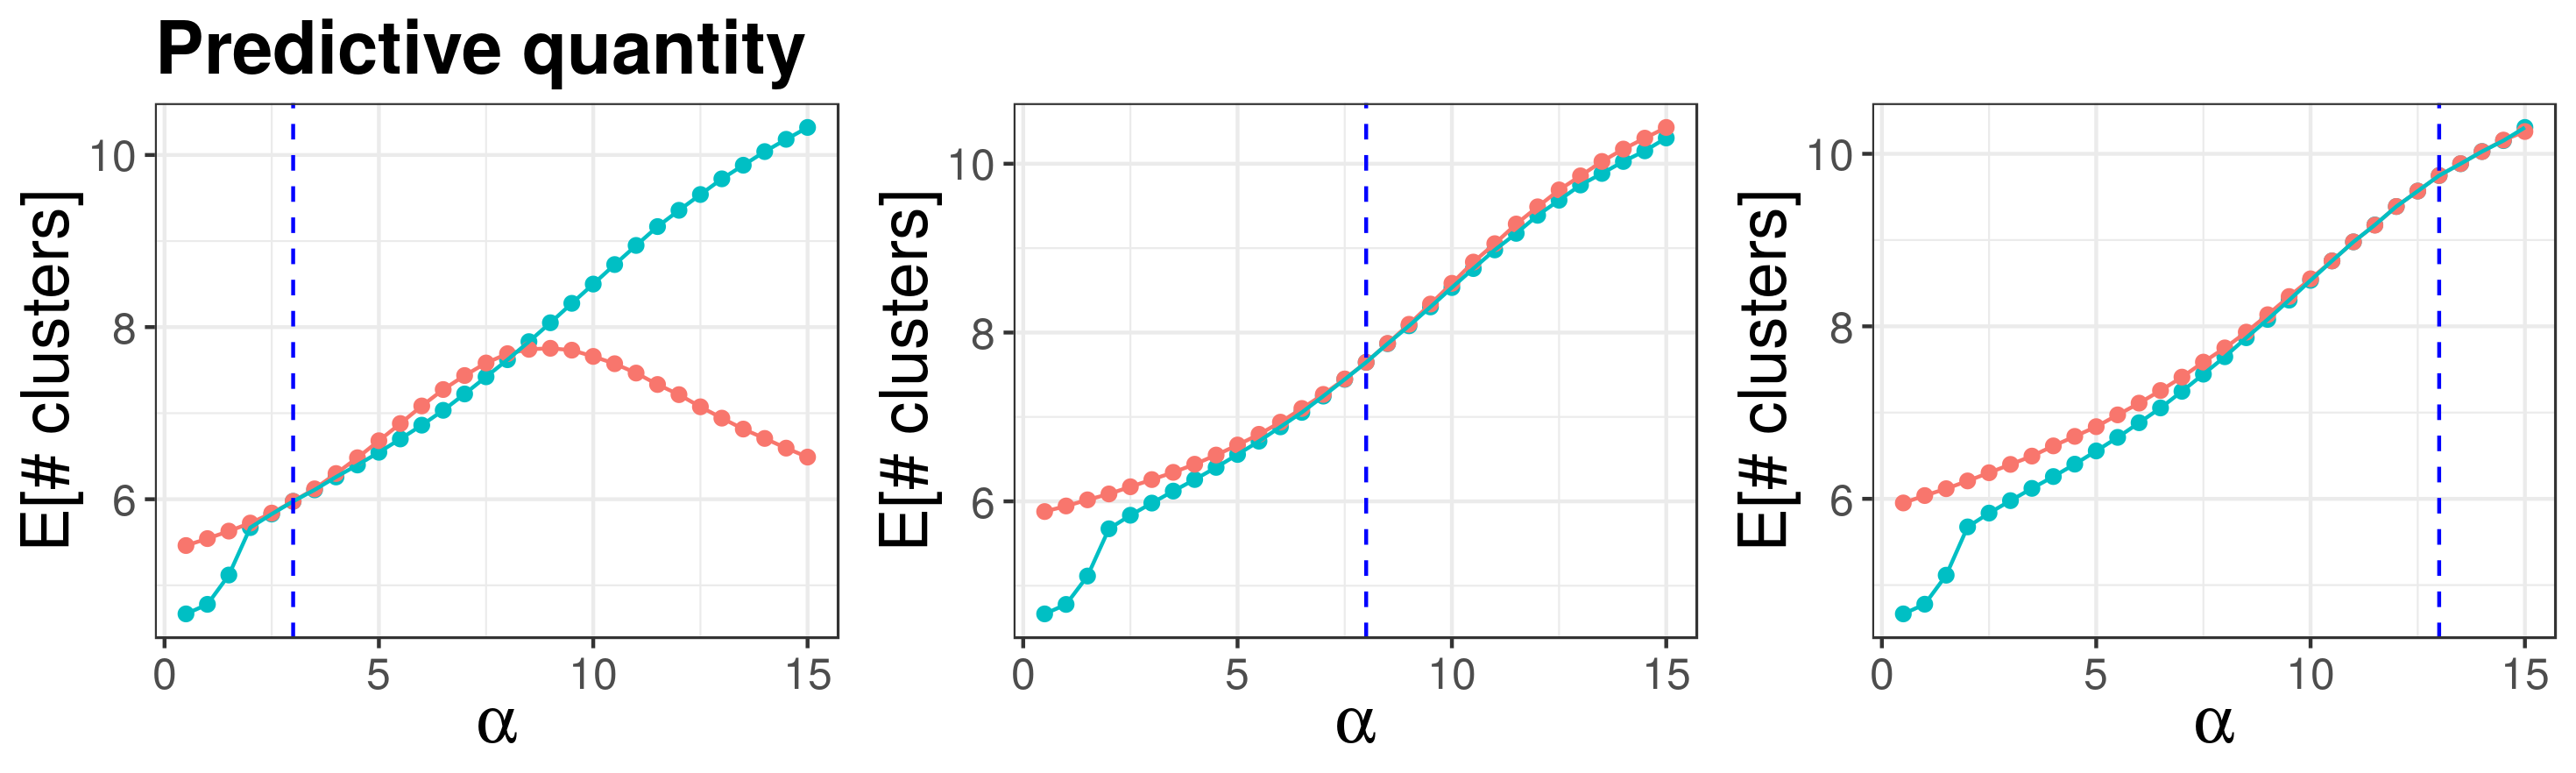
\includegraphics[width=0.98\linewidth,height=0.294\linewidth]{figure/param_sens_plot_thresh_0-1} 
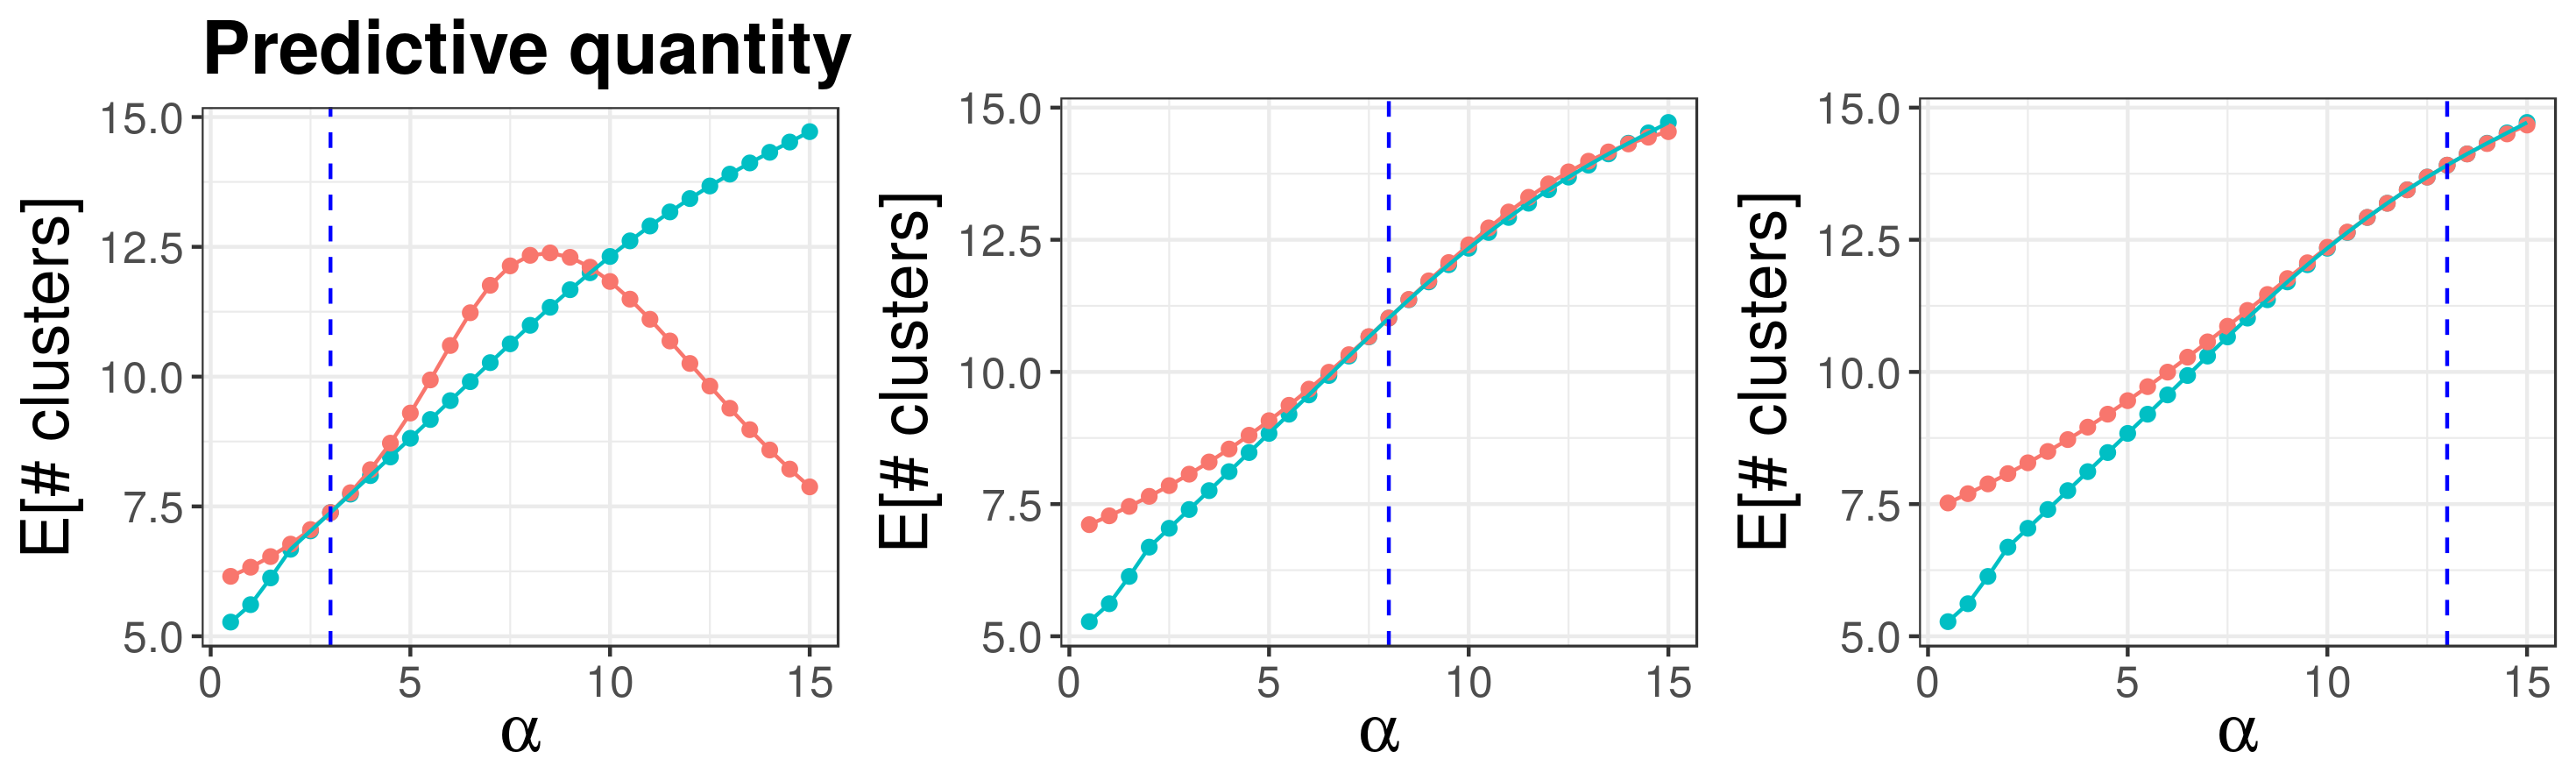
\includegraphics[width=0.98\linewidth,height=0.294\linewidth]{figure/param_sens_plot_thresh_0-2} 

}



\end{knitrout}
\caption{Comparison of in-sample (top) and predictive (bottom) expected number of clusters computed by re-optimization (green) versus linear approximation (orange). 
Vertical line indicates the location of $\alpha_0$, the initial fit. }
\end{figure}

{\bf \large Sensitivity to functional perturbations. }
Suppose we replace the original beta prior $p_0$ with another distribution $p_1$. Then we set our perturbation to be
\vspace{-0.3in}
\begin{align*}
p_c(\nu_k \vert \delta) \propto p_{0}(\nu_k)\left(\frac{p_1(\nu_k)}{p_0(\nu_k)}\right)^\delta
\end{align*}
\vspace{-0.3in}

and evaluate sensitivity to $\delta$:
% \vspace{-0.2in}
% \begin{align}
% \label{eq:expon_perturb}
% 	p_c(\nu_k \vert \delta, \phi) :=
%   \frac{p_{0}(\nu_k)\phi(\nu_k)^\delta}
%        {\int_0^1 p_0(\nu_k')\phi(\nu')^\delta d\nu_k'}.
% \end{align}
% We evaluate the effect of $\delta$:
\vspace{0.1in}
\begin{figure}
\centering

\begin{knitrout}
\definecolor{shadecolor}{rgb}{0.969, 0.969, 0.969}\color{fgcolor}

{\centering 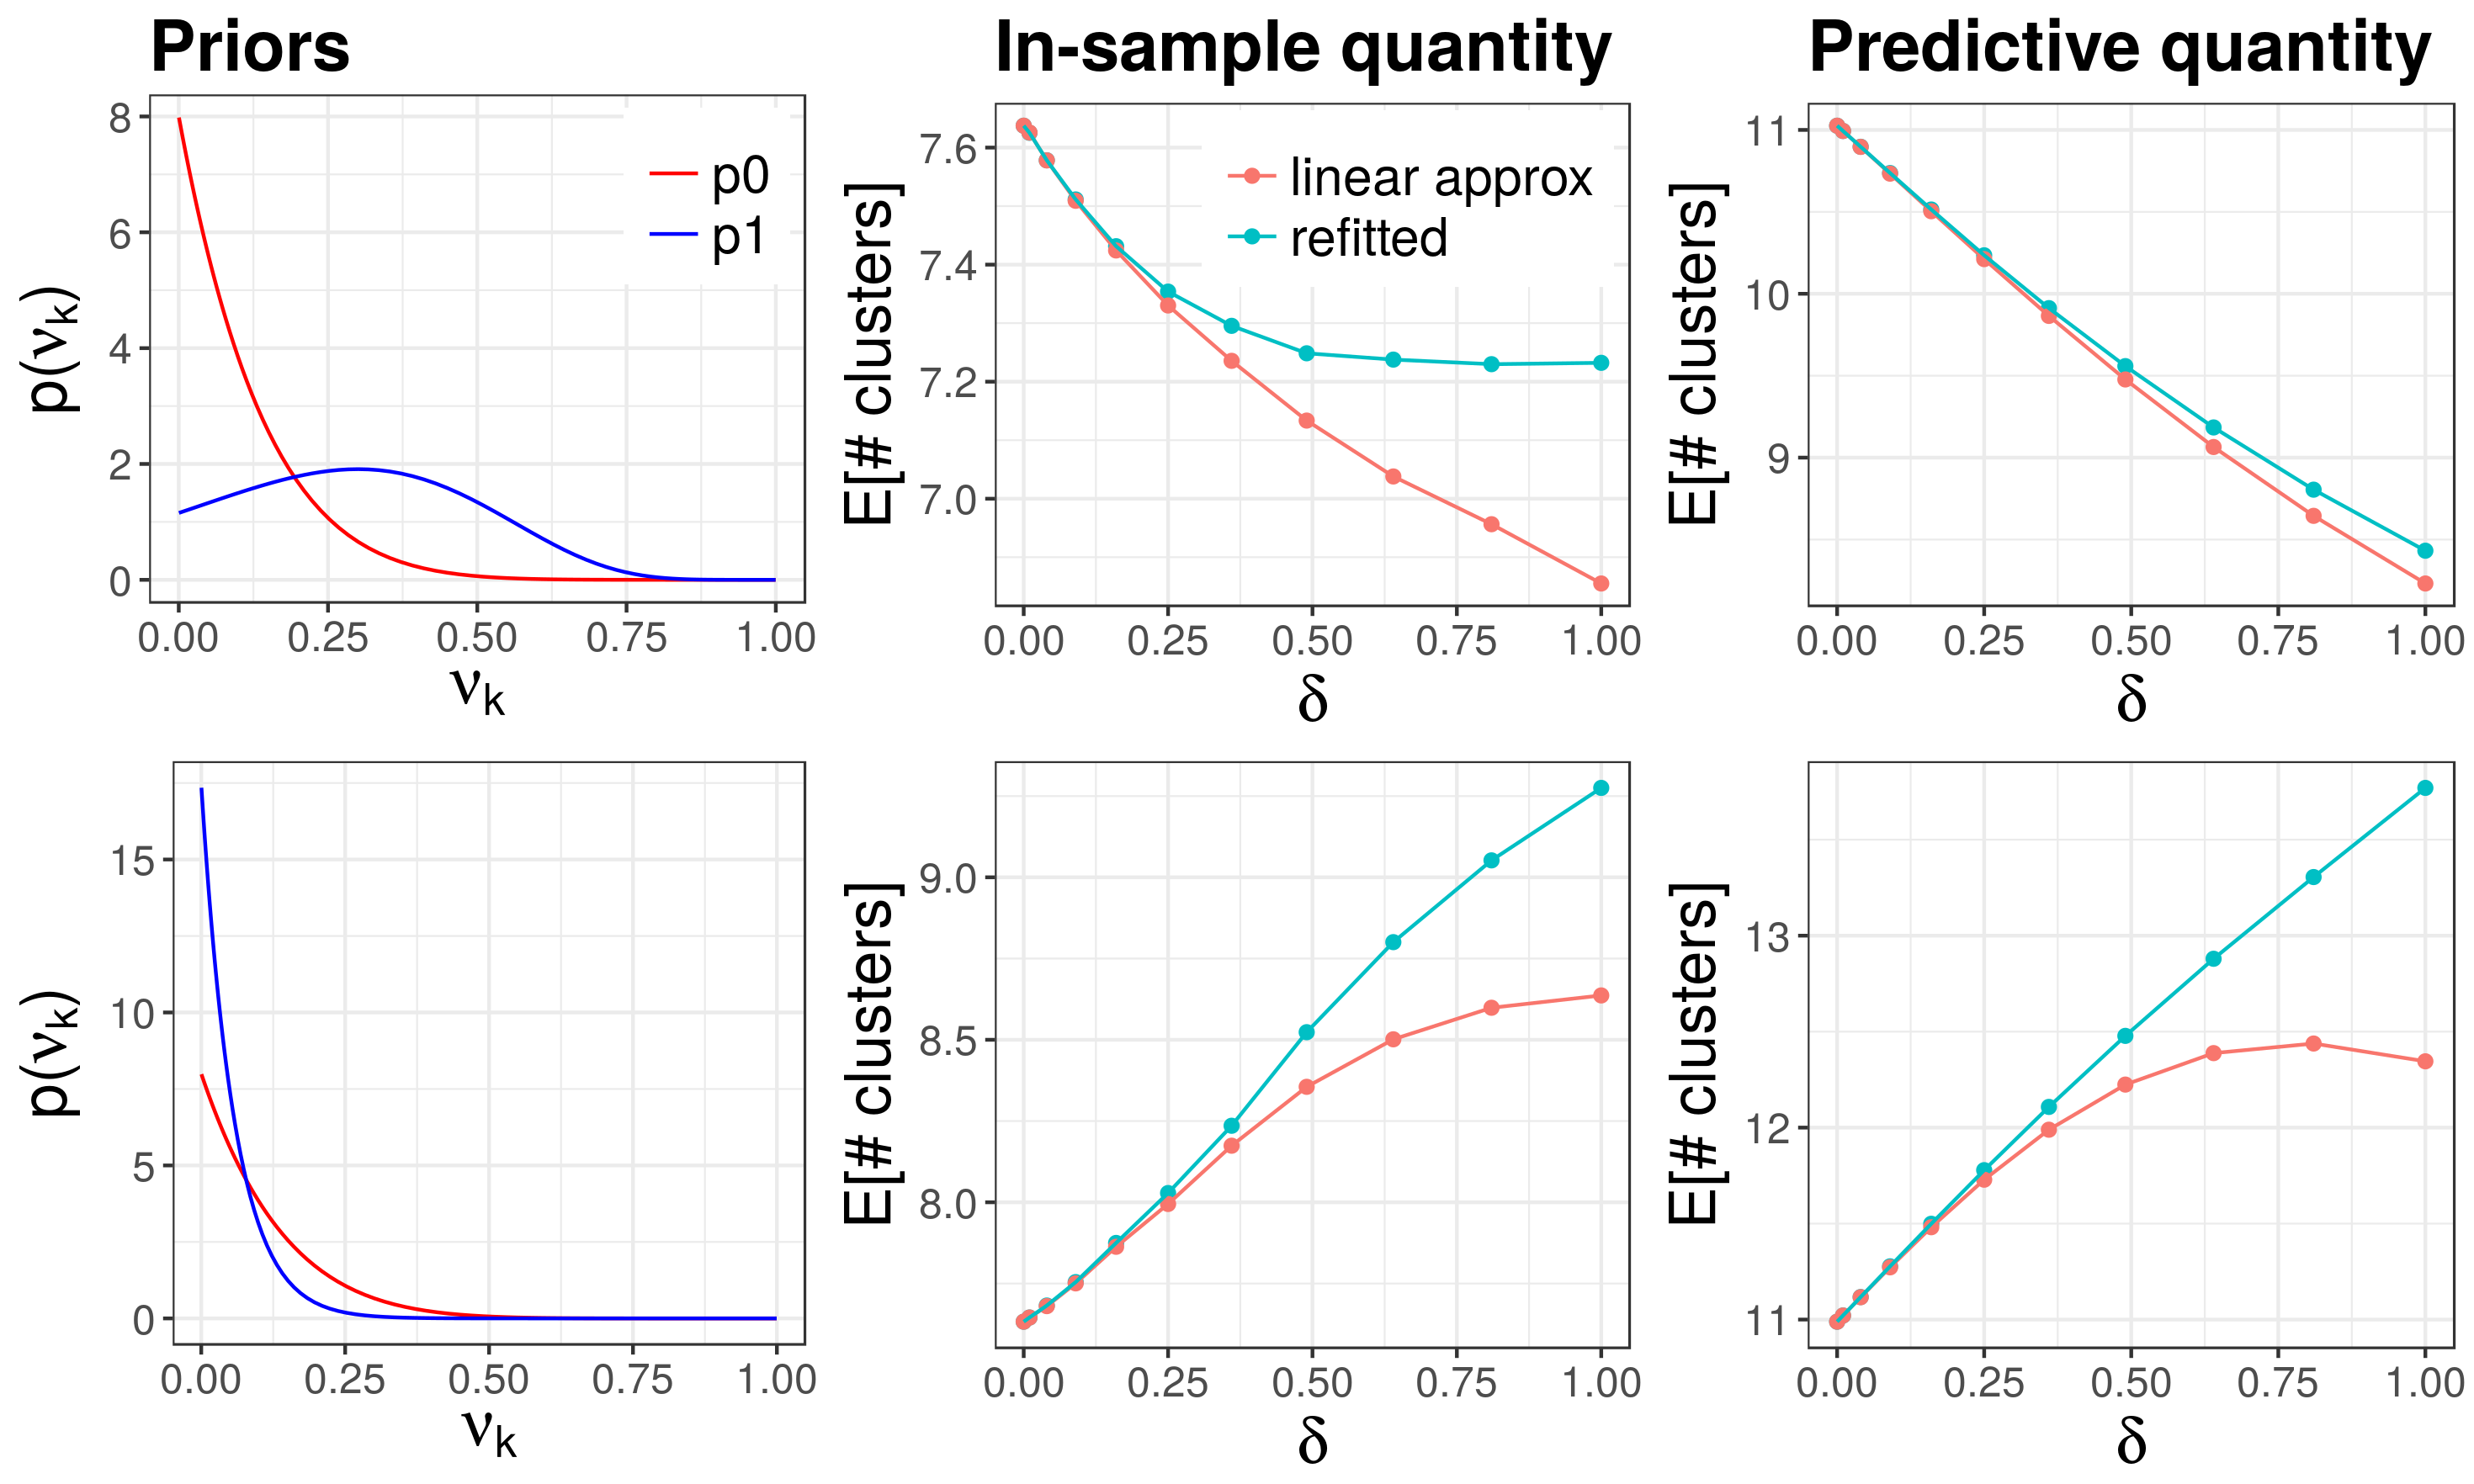
\includegraphics[width=0.98\linewidth,height=0.588\linewidth]{figure/functional_sens_plot_thresh0-1} 

}



\end{knitrout}
\caption{The effect of prior perturbation on the expected number of clusters. Left column: the original prior $p_0$ in red, the perturbed prior $p_1$ in blue. Middle: linearly approximated vs.
re-fitted in-sample expected number of clusters. Right: linearly approximated vs. re-fitted predictive expected number of clusters.}
\end{figure}

% Because we have used a multiplicative perturbation, $f_\eta$
% is linear in $\epsilon$. We might expect this to improve the fidelity of a
% linear approximation. 
\begin{mdframed}[style=MyFrame]
%%%%%%%%%%%%%%%%%%%%%%%%%%%%%%%%%
%%%%%%%%%%%%%%%%%%
\vspace{-0.6in}
\section*{Conclusion}
\vspace{-0.3in}
%%%%%%%%%%%%%%%%%%
%%%%%%%%%%%%%%%%%%%%%%%%%%%%%%%%%

\begin{itemize}

\item {\bf Our linear approximation provides a fast alternative to re-evaluating the full model after changing the BNP prior. }

\item We applied our approximation to both parametric and functional perturbations of the stick-breaking prior.

\item We attempted to improve the linearity by approximating only the dependence of the optimal variational parameters on prior parameters.

\end{itemize}
\end{mdframed}

{\bf Our code: }\newline
Paragami: general library for sensitivity analysis in optimization problems\newline
{\color{blue} https://github.com/rgiordan/paragami}

Code to evaluate BNP sensitivity as shown here: \newline
{\color{blue} https://github.com/Runjing-Liu120/sensitivity\_to\_stick\_breaking\_in\_BNP}


\end{minipage}\\

\begin{center}

{\bf Contact: } rgiordano@berkeley.edu, runjing\_liu@berkeley.edu

\end{center}

\end{document}
